
\centerline{\textbf{ \LARGE Memory Management Basics}}

% ----------------------------------------------------------------------------

\begin{enumerate}

  \item Memory  unit (hardware) : https://www.geeksforgeeks.org/memory-management-in-operating-system/ \\
     \begin{myTableStyle}
      \begin{tabular}{ |m{5cm}|m{10cm}| } \hline
          Logical(virtual) address      &      CPU generates logical addresses. It is assigned by the compiler.    \\ \hline
          Physical address(main memory) &      Seen by the memory unit.    \\ \hline
          Relocation(mapping)           &      Converts logical to physical address.  \\ \hline
          Sharing                       &      Sharing of code between 2 processes. \\ \hline
          Protection                    &      Processes do not corrupt each other's data in main memory. \\ \hline
          Loader                        &      Loads a process in main memory. \\ \hline
      \end{tabular}
    \end{myTableStyle}
  \vspace{0.08in}

  \item Logical vs Physical Address \\
     \begin{myTableStyle}
      \begin{tabular}{ |m{2cm}|c|c| } \hline
                       &  Address bits    & Address Space          \\ \hline
          Physical     &  22    &   \(2^{22} \) words  \\ \hline
          Logical      &  31    &   \(2^{31} \) words   \\ \hline
      \end{tabular}
    \end{myTableStyle}
  \vspace{0.08in}

  \item Fixed (static) Partitioning. https://www.geeksforgeeks.org/fixed-or-static-partitioning-in-operating-system/

  \begin{figure}[h]
      \centering   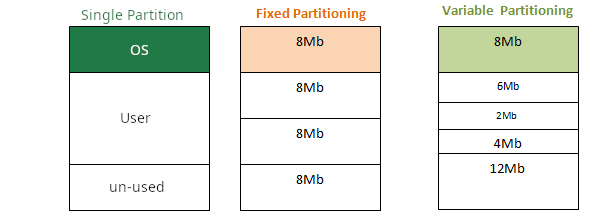
\includegraphics[scale=3]{./images/contigious_partition_01.jpeg}
  \end{figure}

  \begin{enumerate}
    \item Types : Single and Multi partition scheme
    \item Contiguous allocation
    \item Memory is divided into multiple partitions.
    \item Simple, easy to implement
    \item Internal and Ext fragmentation
    \item Suitable for fixed number of processes, ex batch processing
    \item process size is limited by partition size
    \item Limits degree of Multiprogramming
    \item Phy addr = base addr + log addr
    \item First, best, worst fit
    \item No data sharing between processes
  \end{enumerate}

  \begin{minipage}{\linewidth}
    \item Non-contiguous Memory Allocation:
    \begin{enumerate}
      \item External fragmentation : many free pieces in memory. Can not be allocated to a process since they are not contiguous.
      \item Solution to external fragmentation is to use non-contiguous memory allocation techniques.
      \item Paging, segmentation, Paging and segmentation combined.
    \end{enumerate}
  \end{minipage}

\end{enumerate}

% ----------------------------------------------------------------------------

% ----------------------------------------------------------------------------

% ----------------------------------------------------------------------------

% ----------------------------------------------------------------------------

% ----------------------------------------------------------------------------

% ----------------------------------------------------------------------------

% ----------------------------------------------------------------------------

% ----------------------------------------------------------------------------
